\documentclass[pdf,aspectratio=169]{beamer}
\usepackage[]{hyperref,graphicx,siunitx,booktabs,lmodern}
\usepackage{physics}
\usepackage{em-commands}
\mode<presentation>{\usetheme{EM}}

%Question Numbering
\newcounter{questionnumber}
\newcommand{\qnum}{%
	\stepcounter{questionnumber}%
	Q\arabic{questionnumber}
}
\resetcounteronoverlays{questionnumber}

\graphicspath{ {../Images/} }

\sisetup{per-mode=symbol}

\tikzstyle{plate}=[draw, very thick, minimum width=4cm, minimum height=1cm, fill=gray!40, anchor=south]

%preamble
\title{Current Events: Magnetostatics}
\date{October 24, 2018}
\author{Jed Rembold}

\begin{document}
\renewcommand{\theenumi}{\Alph{enumi}}

\begin{frame}{Announcements}
	\begin{itemize}
		\item Homework 8 posted! Due on Monday!
			\begin{itemize}
				\item Should be ok to do all but maybe 1 or 2 problems after today
			\end{itemize}
		\item I'm working on grade reports
		\item Physics Club tomorrow
			\begin{itemize}
				\item Still working on solving mazes?
			\end{itemize}
		\item Read 5.2 for Friday
	\end{itemize}
\end{frame}

\begin{frame}{\qnum}
	A negative charge, $-q$, is moving in the $+\xhat$ direction when it encounters a region of constant magnetic field pointing in the $-\yhat$ direction. What is the direction of the initial net force on the charge?
	\begin{enumerate}
		\item $+\yhat$
		\item $-\yhat$
		\item \alert<2>{$+\zhat$}
		\item $-\zhat$
	\end{enumerate}
\end{frame}

\begin{frame}{\qnum}
	A proton, $q=+e$, is released from rest in a uniform $\ef$ and uniform $\mf$. $\ef$ points up, and $\mf$ points into the page. Which of the paths will the proton initially follow?
	\begin{center}
		\begin{tikzpicture}
			\foreach \x in {1,2,...,4}{
				\foreach \y in {1,2,...,4}{
					\node at (\x,\y-.5) {$\otimes$};
				}
				\draw[very thick, -latex, Red] (\x-.5, 0) -- +(0,4);
			}
			\node[math, Red, left] at (.5,4) {\ef};
			\node[math, right] at (4,3.5) {\mf};
		\end{tikzpicture}
		\hspace{2cm}
		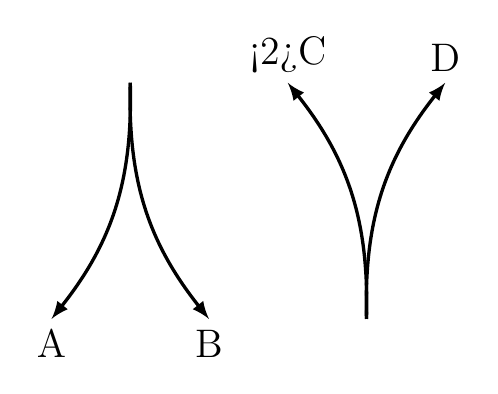
\begin{tikzpicture}
			\path[very thick, -latex]
				(1,3) edge[bend left=20] node[at end,below,font=\Large]{A} (0,0)
				(1,3) edge[bend right=20] node[at end,below,font=\Large]{B} (2,0)
				(4,0) edge[bend right=20] node[at end,above,font=\Large]{\alert<2>{C}} (3,3)
				(4,0) edge[bend left=20] node[at end,above,font=\Large]{D} (5,3);
		\end{tikzpicture}
	\end{center}
\end{frame}

\begin{frame}{\qnum}
	A positively charged particle moving upwards with speed $v$ enters a region with uniform $\mf$ to the left and uniform $\ef$ into the page. What is the direction of $\force_{net}$ on the particle the instant it enters the region?
	\begin{columns}
		\column{0.5\textwidth}
		\begin{enumerate}
			\item To the left
			\item To the right
			\item Into the page
			\item \alert<2>{Not enough info to say}
		\end{enumerate}
		\column{0.5\textwidth}
		\begin{center}
			\begin{tikzpicture}
				\foreach \y in {0,1,...,3}{
					\foreach \x in {0,1,...,4}{
						\node[Red] at (\x,\y) {$\otimes$};
					}
					\draw[very thick, -latex] (4,\y-.5) -- +(-4,0);
				}
				\node[math,right] at (4,2.5) {\mf};
				\node[Red,math,left] at (0,3) {\ef};

				\draw[latex-,orange,ultra thick] (2,-.6) --+(0,-1) node[right,math] {\vel};
			\end{tikzpicture}
		\end{center}
	\end{columns}
\end{frame}

\begin{frame}{\qnum}
	A box of mass $m$ is attached via a rope of length $\ell$ to a central point. 
	It is spinning at a constant angular speed $\omega$.
	No other forces are present.
	What is the work done by the tension in the rope over one complete revolution?
	\begin{columns}
		\column{0.5\textwidth}
		\begin{enumerate}
			\item \alert<2>{$0$}
			\item $m\omega^2\ell$
			\item $2m\omega^2\pi\ell$
			\item $m\omega^2\pi\ell^2$
		\end{enumerate}
		
		\column{0.5\textwidth}
		\begin{center}
			\begin{tikzpicture}
				\draw[dashed, -latex] (0,0) circle (2.5);
				\begin{scope}[rotate=45]
					\draw[very thick] (0,0) -- node[midway,above,math] {\ell} +(0,-2) node[block=Red, anchor=north] {m};
				\end{scope}
			\end{tikzpicture}
		\end{center}
		
	\end{columns}
\end{frame}

\begin{frame}{\qnum}
	Positive ions flow right through a liquid, while negative ions flow left. The spatial density and speed of both ion types are identical. Is there a net current through the liquid?
	\begin{enumerate}
		\item \alert<2>{Yes, to the right}
		\item Yes, to the left
		\item No
		\item Not enough info is given
	\end{enumerate}
\end{frame}

\begin{frame}{\qnum}
	A uniform current $\cur$ flows through the surface to the left in the direction indicated. What is the surface current density, $\scd$?
	\begin{columns}
		\column{0.5\textwidth}
		\begin{center}
			\tdplotsetmaincoords{70}{110}
			\begin{tikzpicture}[tdplot_main_coords]
				\fill[cyan,opacity=0.5,xzplane=0] (0,0) rectangle +(2,5);
				\draw (0,0,0) -- +(5,0,0);
				\fill[cyan,opacity=0.5,xyplane=0] (0,0) rectangle +(2,5);
				\fill[cyan,opacity=0.5,xzplane=2] (0,0) rectangle +(2,5);
				\draw (0,2,0) -- +(5,0,0);
				\draw[very thick] (5,0,2) -- ++(0,0,-2) node[midway,left]{$\ell$} -- ++(0,2,0) node[midway,below]{$\ell$} -- ++(0,0,2) node[midway,right]{$\ell$};
				\draw[ultra thick, -latex, Red] (4,1,0) -- +(3,0,0) node[below,math] {\cur};
			\end{tikzpicture}
		\end{center}
		\column{0.5\textwidth}
		\begin{enumerate}
			\item $\displaystyle \frac{\cur}{\ell^3}$
			\item \alert<2>{$\displaystyle \frac{\cur}{3\ell}$}
			\item $\displaystyle \frac{\cur}{\ell}$
			\item $\displaystyle 3\ell \cur$
		\end{enumerate}
	\end{columns}
\end{frame}

\begin{frame}{\qnum}
	The volume current density is defined in terms of the differential:
	\[\vcd = \dv{\cur}{a_\perp}\]
	When is it ok to determine the volume current density by taking the ratio of the current to the cross-sectional area?
	\[\vcd \overset{?}{=} \frac{\cur}{A}\]
	\begin{enumerate}
		\item Never
		\item Always
		\item When $\cur$ is uniform
		\item \alert<2>{When $\cur$ is uniform and $A$ is $\perp$ to $\cur$}
	\end{enumerate}
\end{frame}


%\begin{frame}{\qnum}
	%A ``ribbon'' (width $a$) of surface current flows with surface current density $\scd$. Right next to it is a second identical ribbon of current. Viewed collectively, what is the new total surface current density?
	%\begin{columns}
		%\column{0.5\textwidth}
		%\begin{enumerate}
			%\item 0
			%\item $2\scd$
			%\item $\scd/2$
			%\item Something else
		%\end{enumerate}
		%\column{0.5\textwidth}
		%\begin{center}
			%\tdplotsetmaincoords{70}{110}
			%\begin{tikzpicture}[tdplot_main_coords]
				%\draw[very thick, fill=blue!20, xyplane=0] (0,0) rectangle +(4,2);
				%\draw[very thick, fill=blue!20, xyplane=0] (0,2) rectangle +(4,2);
				%\draw[Red, very thick, -latex, xyplane=0] (1,1) -- +(2,0);
				%\draw[Red, very thick, -latex, xyplane=0] (1,3) -- +(2,0);
			%\end{tikzpicture}
		%\end{center}
		
	%\end{columns}
%\end{frame}


\end{document}
